\section{Fonctionnalités}
\sectitle{Réflexions préliminaires et fonctionnalités}

\begin{frame}
    \frametitle{Réflexions préliminaires}

    \begin{itemize}
        \item Définition des besoins du site (\textbf{réunions hebdomadaires})
        \item Analyse des améliorations par rapport à l’ancien site
        \item Étude de faisabilité en lien avec le \textbf{RGPD}
    \end{itemize}
    \bigskip
    
    Toutes ces réflexions nous ont permis de définir les fonctionnalités essentielles pour ce nouveau site.
\end{frame}

\begin{frame}
    \frametitle{Les fonctionnalités du site (1/2)}

    Voici les fonctionnalités retenues : 

    \begin{itemize}
	\item \textbf{Page d'accueil}
        \item \textbf{Présentation de l’association} et de son histoire
        \item \textbf{Gestion des événements et actualités} :  mise en ligne d'événements, inscriptions et suivi...
        \item \textbf{Boutique en ligne} : adhésion et produits dérivés
    \end{itemize}
\end{frame}

\begin{frame}
    \frametitle{Les fonctionnalités du site (2/2)}

    Mais également : 

    \begin{itemize}
        \item \textbf{Galerie photo} : photos souvenirs des événements, photos des bureaux...
        \item \textbf{Espace administrateur} : gestion des événements, photos...
        \item \textbf{Système de comptes} : utilisateurs, administrateurs, entreprises...
        \item \textbf{Jeu ludique} inspiré de \textit{Space Invaders} : OFNIvaders
    \end{itemize}
\end{frame}



\section{Maquettage}
\sectitle{Maquettage du site}

\begin{frame}
    \frametitle{Maquettage du site : La maquette manuscrite}

    \begin{minipage}{0.48\textwidth}
        \centering
        \textbf{Esquisse manuscrite} pour organiser les pages, mettre en forme nos idées, tester différentes mises en page...
	\bigskip

	Maquette améliorée au fil des réunions
    \end{minipage}
    \hfill
    \begin{minipage}{0.48\textwidth}
        \centering
        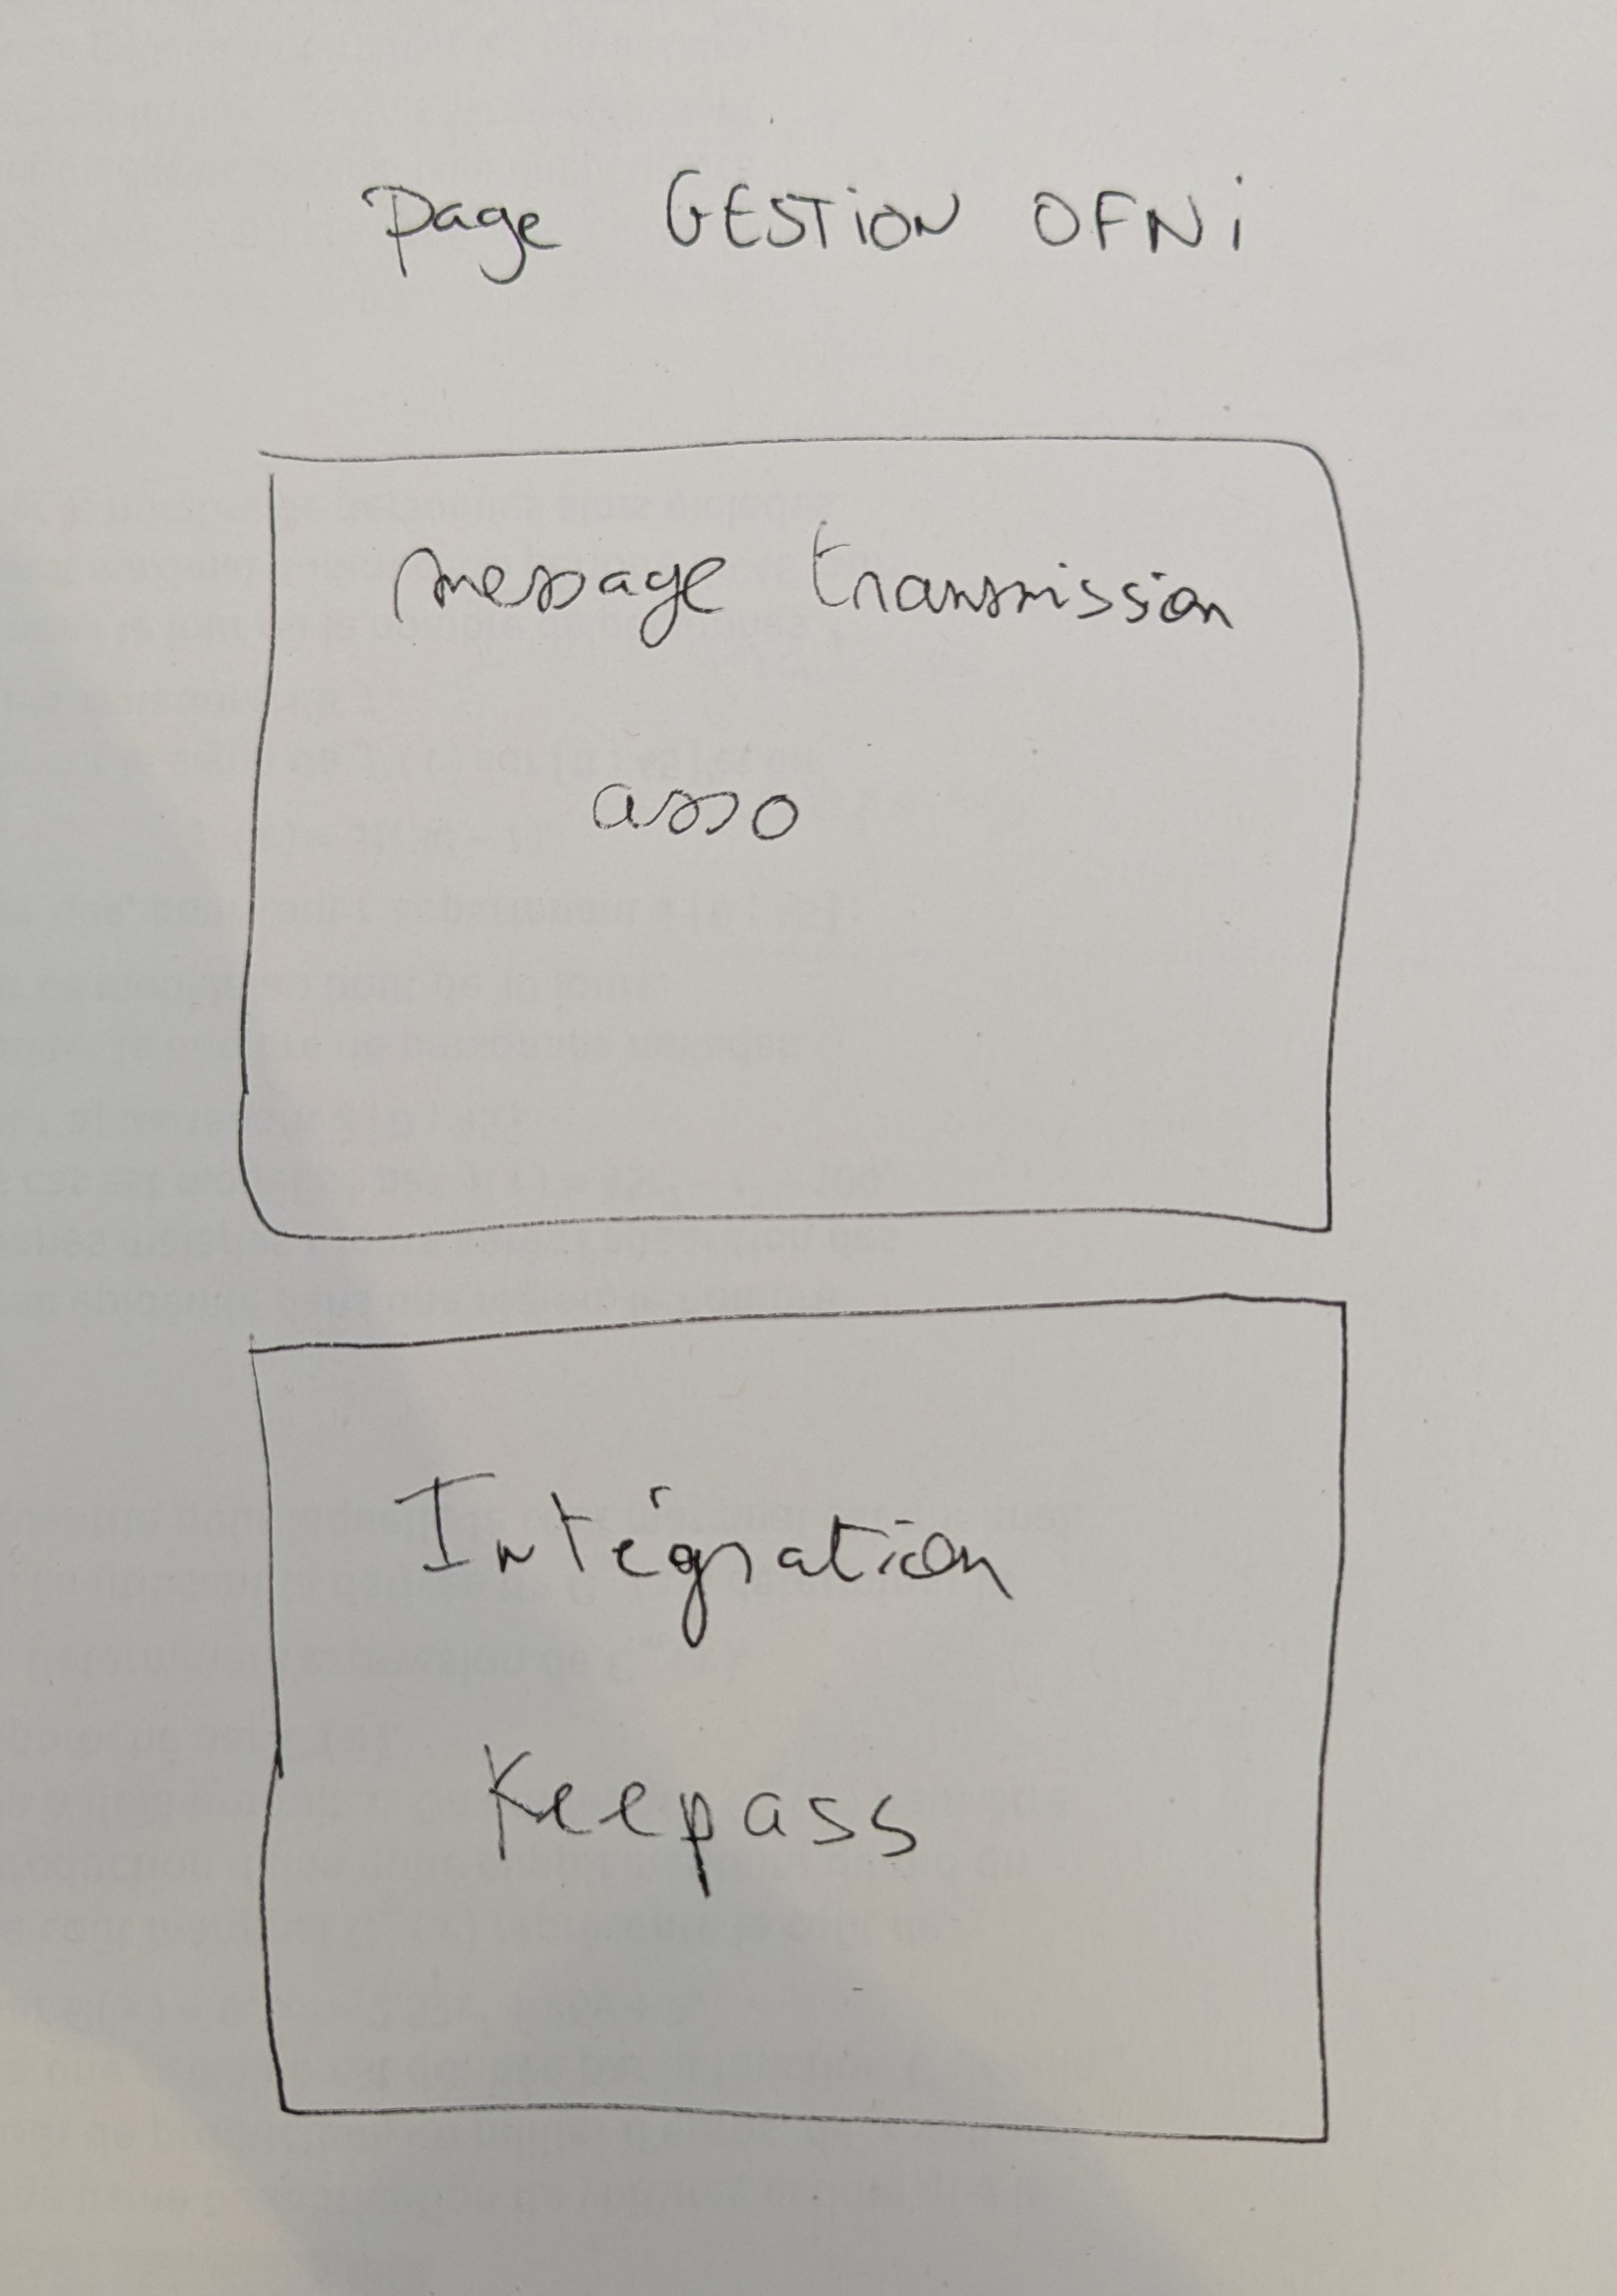
\includegraphics[width=\linewidth]{pictures/maquette.jpg}
        %\captionof{figure}{Maquette numérique}
    \end{minipage}
\end{frame}

\begin{frame}
    \frametitle{Maquettage du site : La maquette numérisée}

    \begin{minipage}{0.48\textwidth}
        \centering
        
\includegraphics[width=\linewidth]{pictures/figma_logo.png}
	Outil pour la numérisation de la maquette
	\bigskip

	\textbf{Maquette numérique} au propre, qui servira de modèle à suivre pour le développement.
    \end{minipage}
    \hfill
    \begin{minipage}{0.48\textwidth}
        \centering
        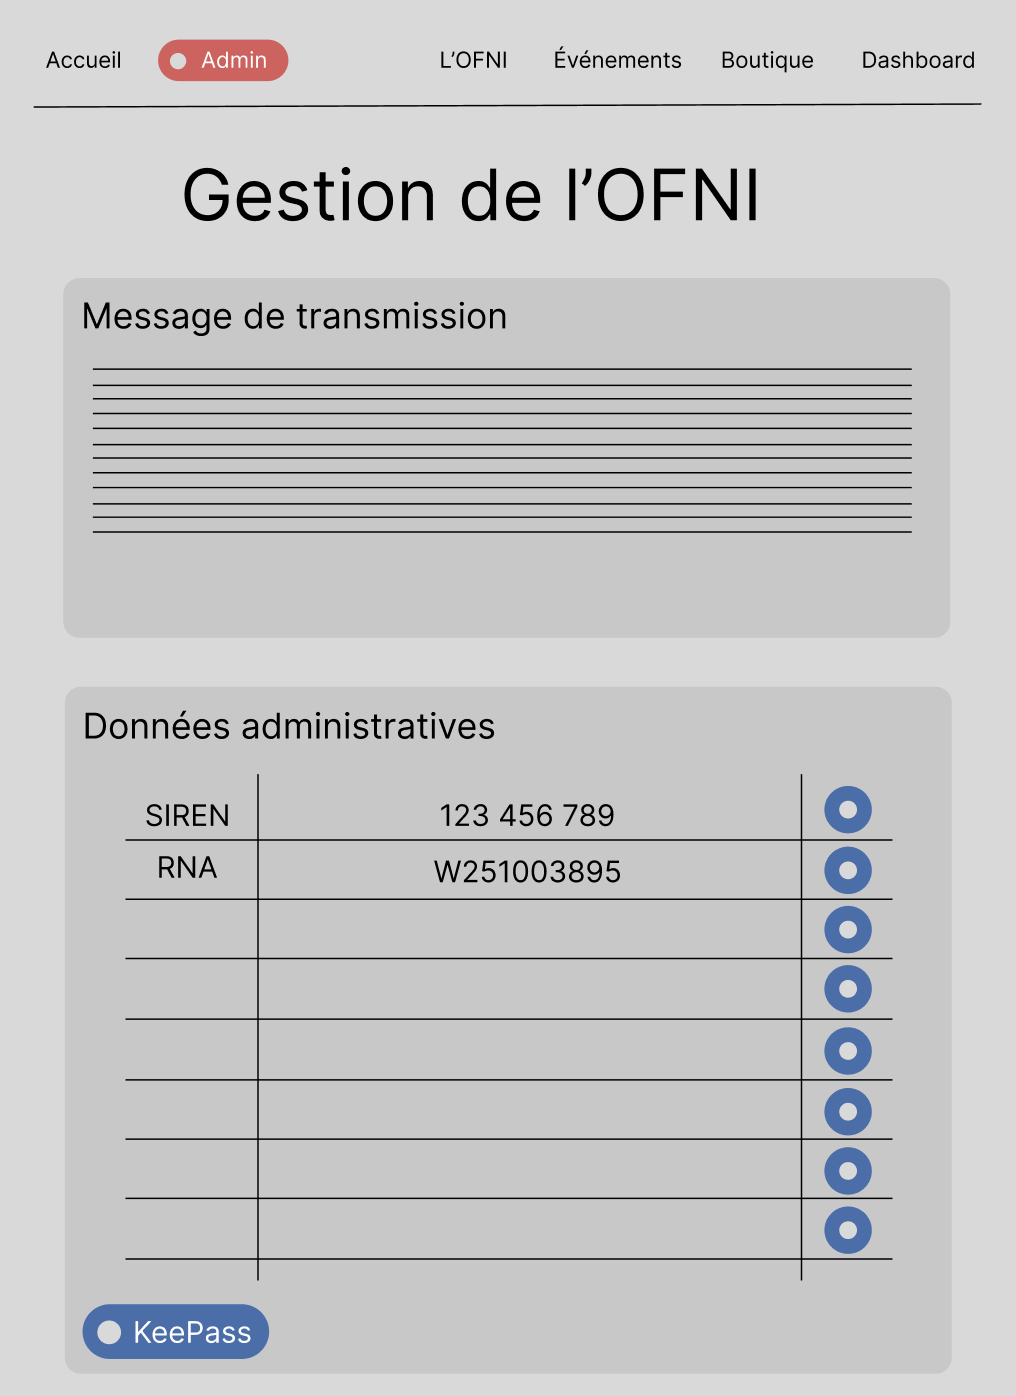
\includegraphics[width=\linewidth]{pictures/figma.png}
        %\captionof{figure}{Maquette numérique}
    \end{minipage}

\end{frame}

